\documentclass[12pt]{article}

\usepackage[utf8]{inputenc}
\usepackage{amsmath}
\usepackage{amsfonts}
\usepackage{graphicx}
\usepackage{subfig}



\begin{document}

Let $x$ and $y$ be random bitstrings and $n$ be the SDM's number of bits; let $x_i$ and $y_i$ be the $i$th bit of $x$ and $y$, respectivelly; and $d(x, y)$ be the Hamming distance.

Applying the law of total probability:

\begin{align}
P(x_i = y_i | d(x, y) \le r) = \sum_{k=0}^{r} P(x_i = y_i | d(x, y) = k \le r) \cdot P(d(x, y) = k | d(x, y) <= r)
\end{align}

We also know that

\begin{align}
P(x_i = y_i | d(x, y) = k) &= \frac{n-k}{n} \\
P(d(x, y) = k | d(x, y) \le r) &= \frac{\binom{n}{k}}{\sum_{j=0}^{r} \binom{n}{j}}
\end{align}

Hence,

\begin{align}
P(x_i = y_i | d(x, y) \le r) = \frac{\sum_{k=0}^{r} \frac{n-k}{n} \binom{n}{k}}{\sum_{j=0}^{r} \binom{n}{j}}
\end{align}

Finally, as $\frac{n-k}{n} \binom{n}{k} = \binom{n-1}{k}$,

\begin{align}
P(x_i = y_i | d(x, y) \le r) = \frac{\sum_{k=0}^{r} \binom{n-1}{k}}{\sum_{k=0}^{r} \binom{n}{k}}
\end{align}

This equation is valid for both ``x at x'' (autoassociative memory) and ``random at x'' (heteroassociative memory). When $n=1,000$ and $r=451$, $P(x_i = y_i | d(x, y) \le r) = p = 0.552905498137$.

\section{Counter bias}

The bias begins in the counters. Let's analyze $i$th counter of a hard location.

Let $s$ be the number of bitstrings written into memory (in our case, $s=10,000$), $h$ be the average number of activated hard locations ($h=1,071.85$), $H$ be the number of hard locations ($H=1,000,000$), and $\text{addr}_i$ be the $i$th bit of the hard location's address. Then,

\begin{align}
P(\text{cnt}_i > 0 | \text{addr}_i = 1) = P(\text{cnt}_i < 0 | \text{addr}i = 0) = \sum_{k=1}^{\theta} X_k > \frac{sh}{2H}
\end{align}

Where $\theta = \frac{sh}{H}$ is the average number of bitstrings written in each hard location, and $X_k \sim \text{Bernoulli}(p)$ (where $p = P(x_i = y_i | d(x, y) \le r)$). Thus, $\sum_{k=1}^{\theta} X_k \sim \text{Binomial} \left( \theta, p \right)$.

Finally, $P(\text{cnt}_i > 0 | \text{addr}_i = 1) = P(\text{cnt}_i < 0 | \text{addr}_i = 0) = \text{Binomial.cdf} \left( \frac{sh}{2H} \right)$.


For ``random at x'', $p=0.5$, $P(\text{cnt}_i > 0 | \text{addr}_i = 1) = P(\text{cnt}_i < 0 | \text{addr}_i = 0) = 0.5$, independently of the parameters. But, for ``x at x'', $p=0.5529$ and the probabilities depend on $s$. For $s=10,000$, they are equal to 0.6362. For $s=20,000$, they are equal to 0.6888. For $s=30,000$, they are equal to 0.7268. The more random bitstrings are written into the memory, the more a hard location to point to itself. See Figure \ref{fig:sdm-corr-prob} --- and notice that I still have to figure out why the mean is correct, but the standard deviation is not. As each of the $n$ counters of a hard location may be equal or not with the same probability, I assumed it would follow a Binomial distribution (and it worked for ``random at x'').

\begin{figure}[h!]
  \centering
  \subfloat[``random at x'']{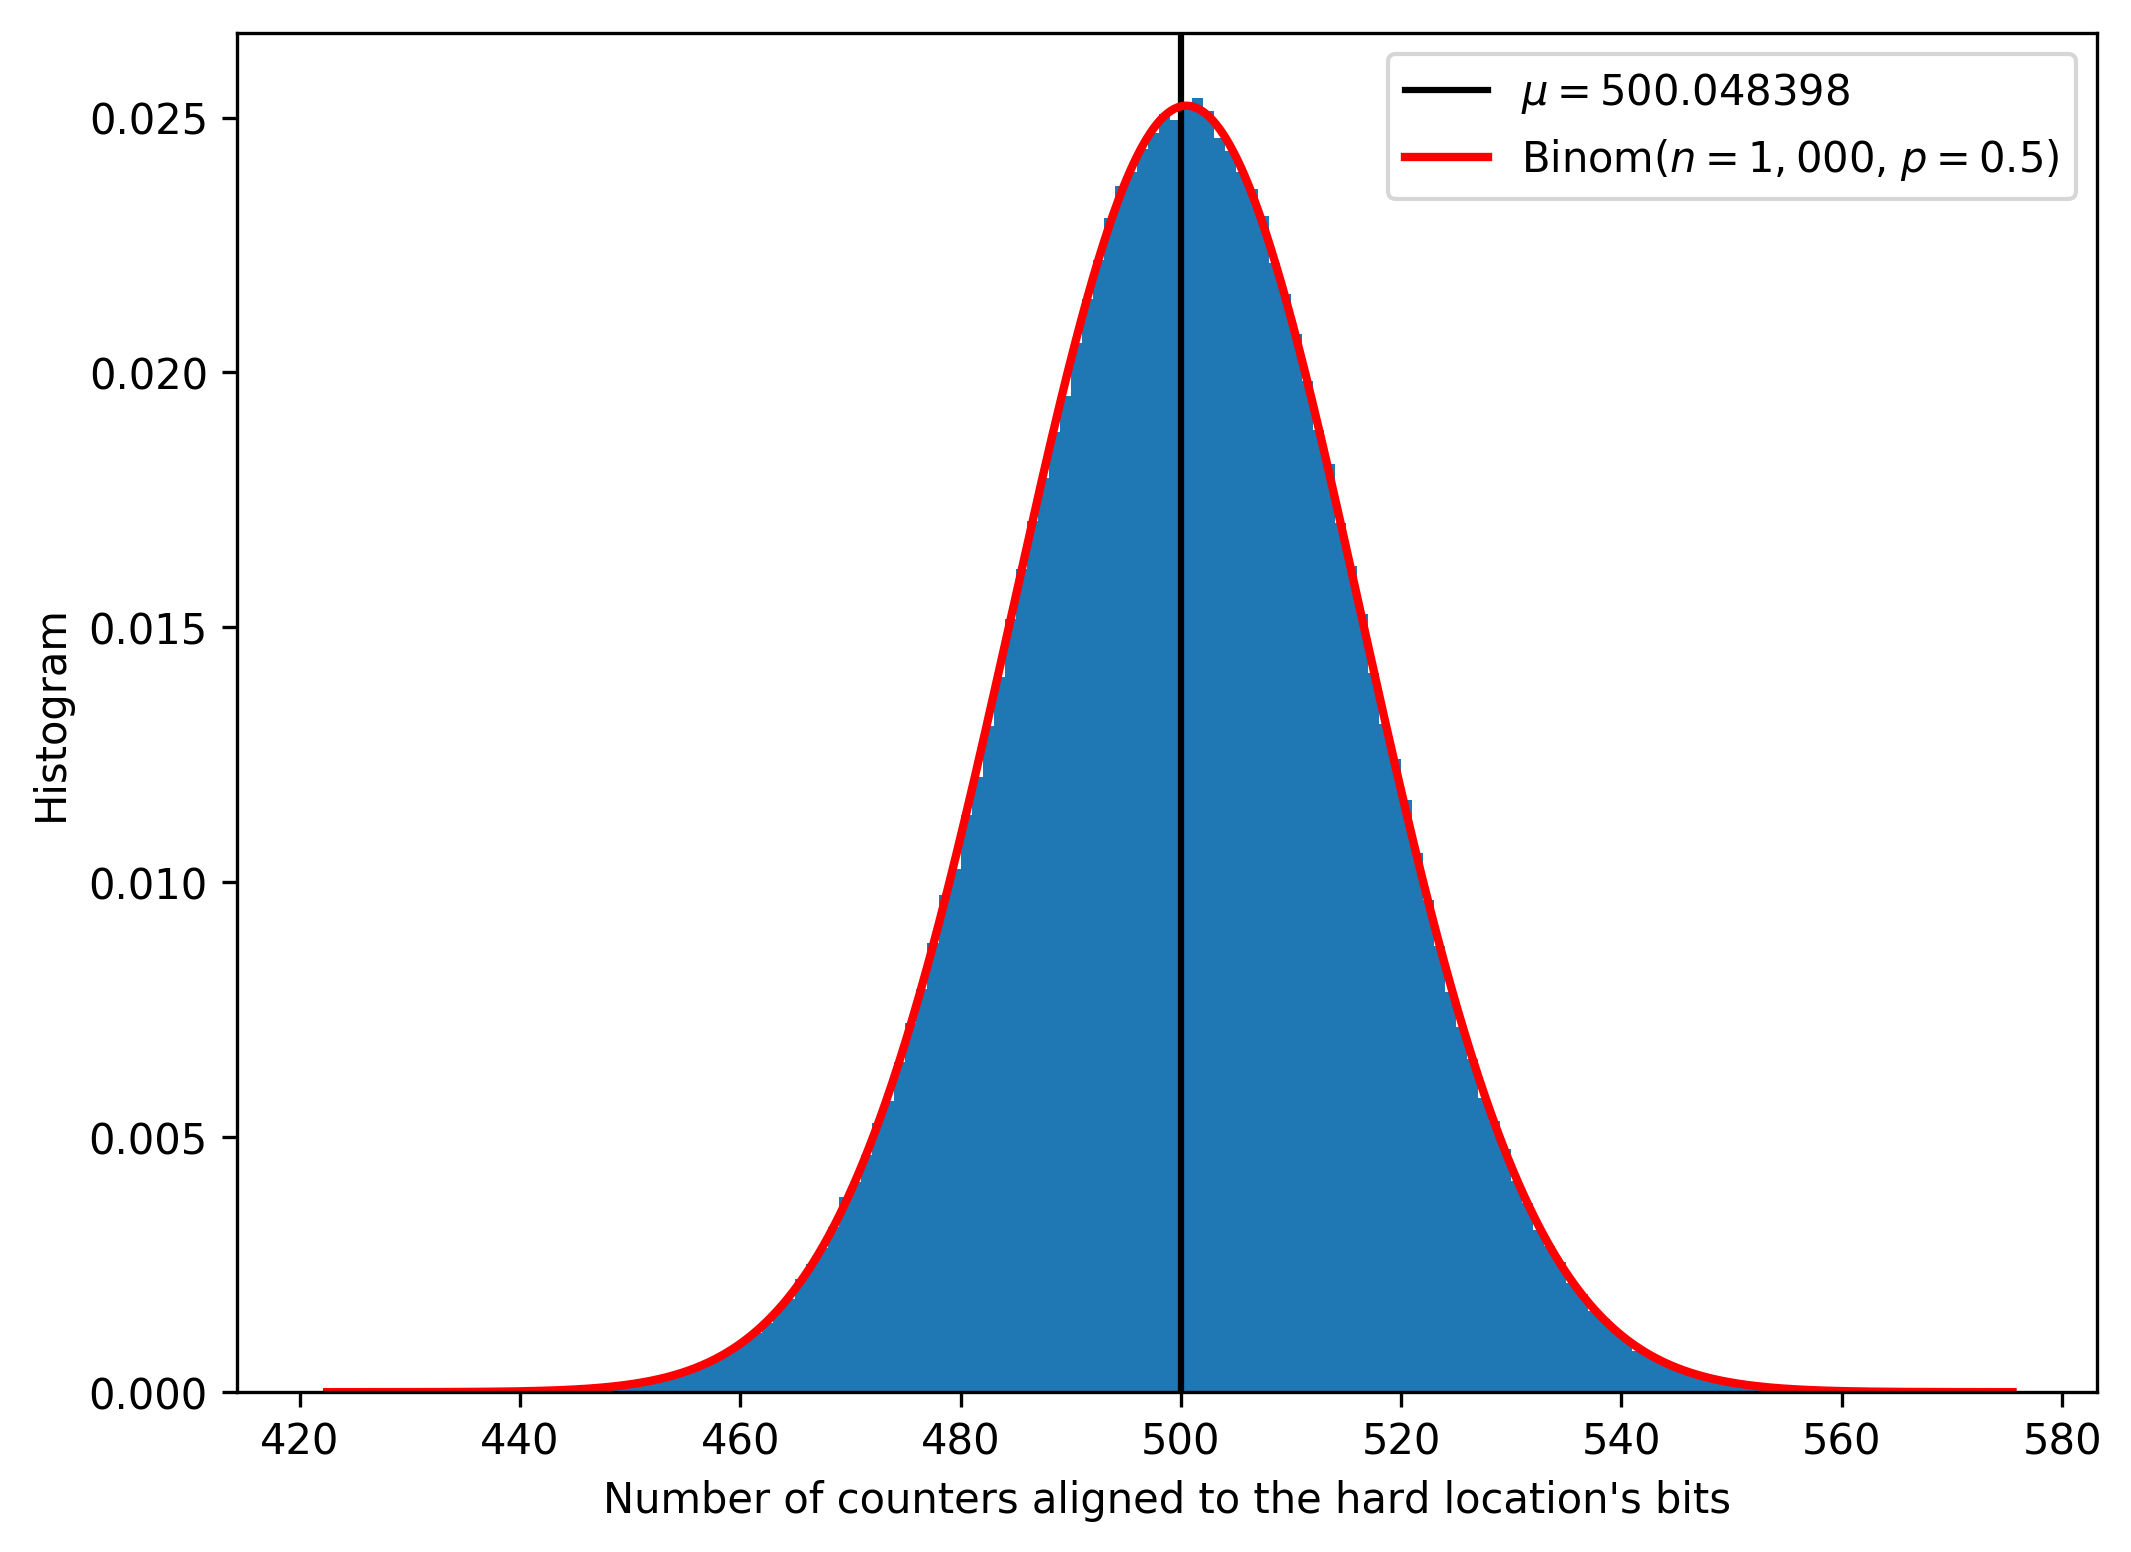
\includegraphics[width=0.5\textwidth]{./images02/autocorrelation/random_at_x_counters.png}}
  \subfloat[``x at x'']{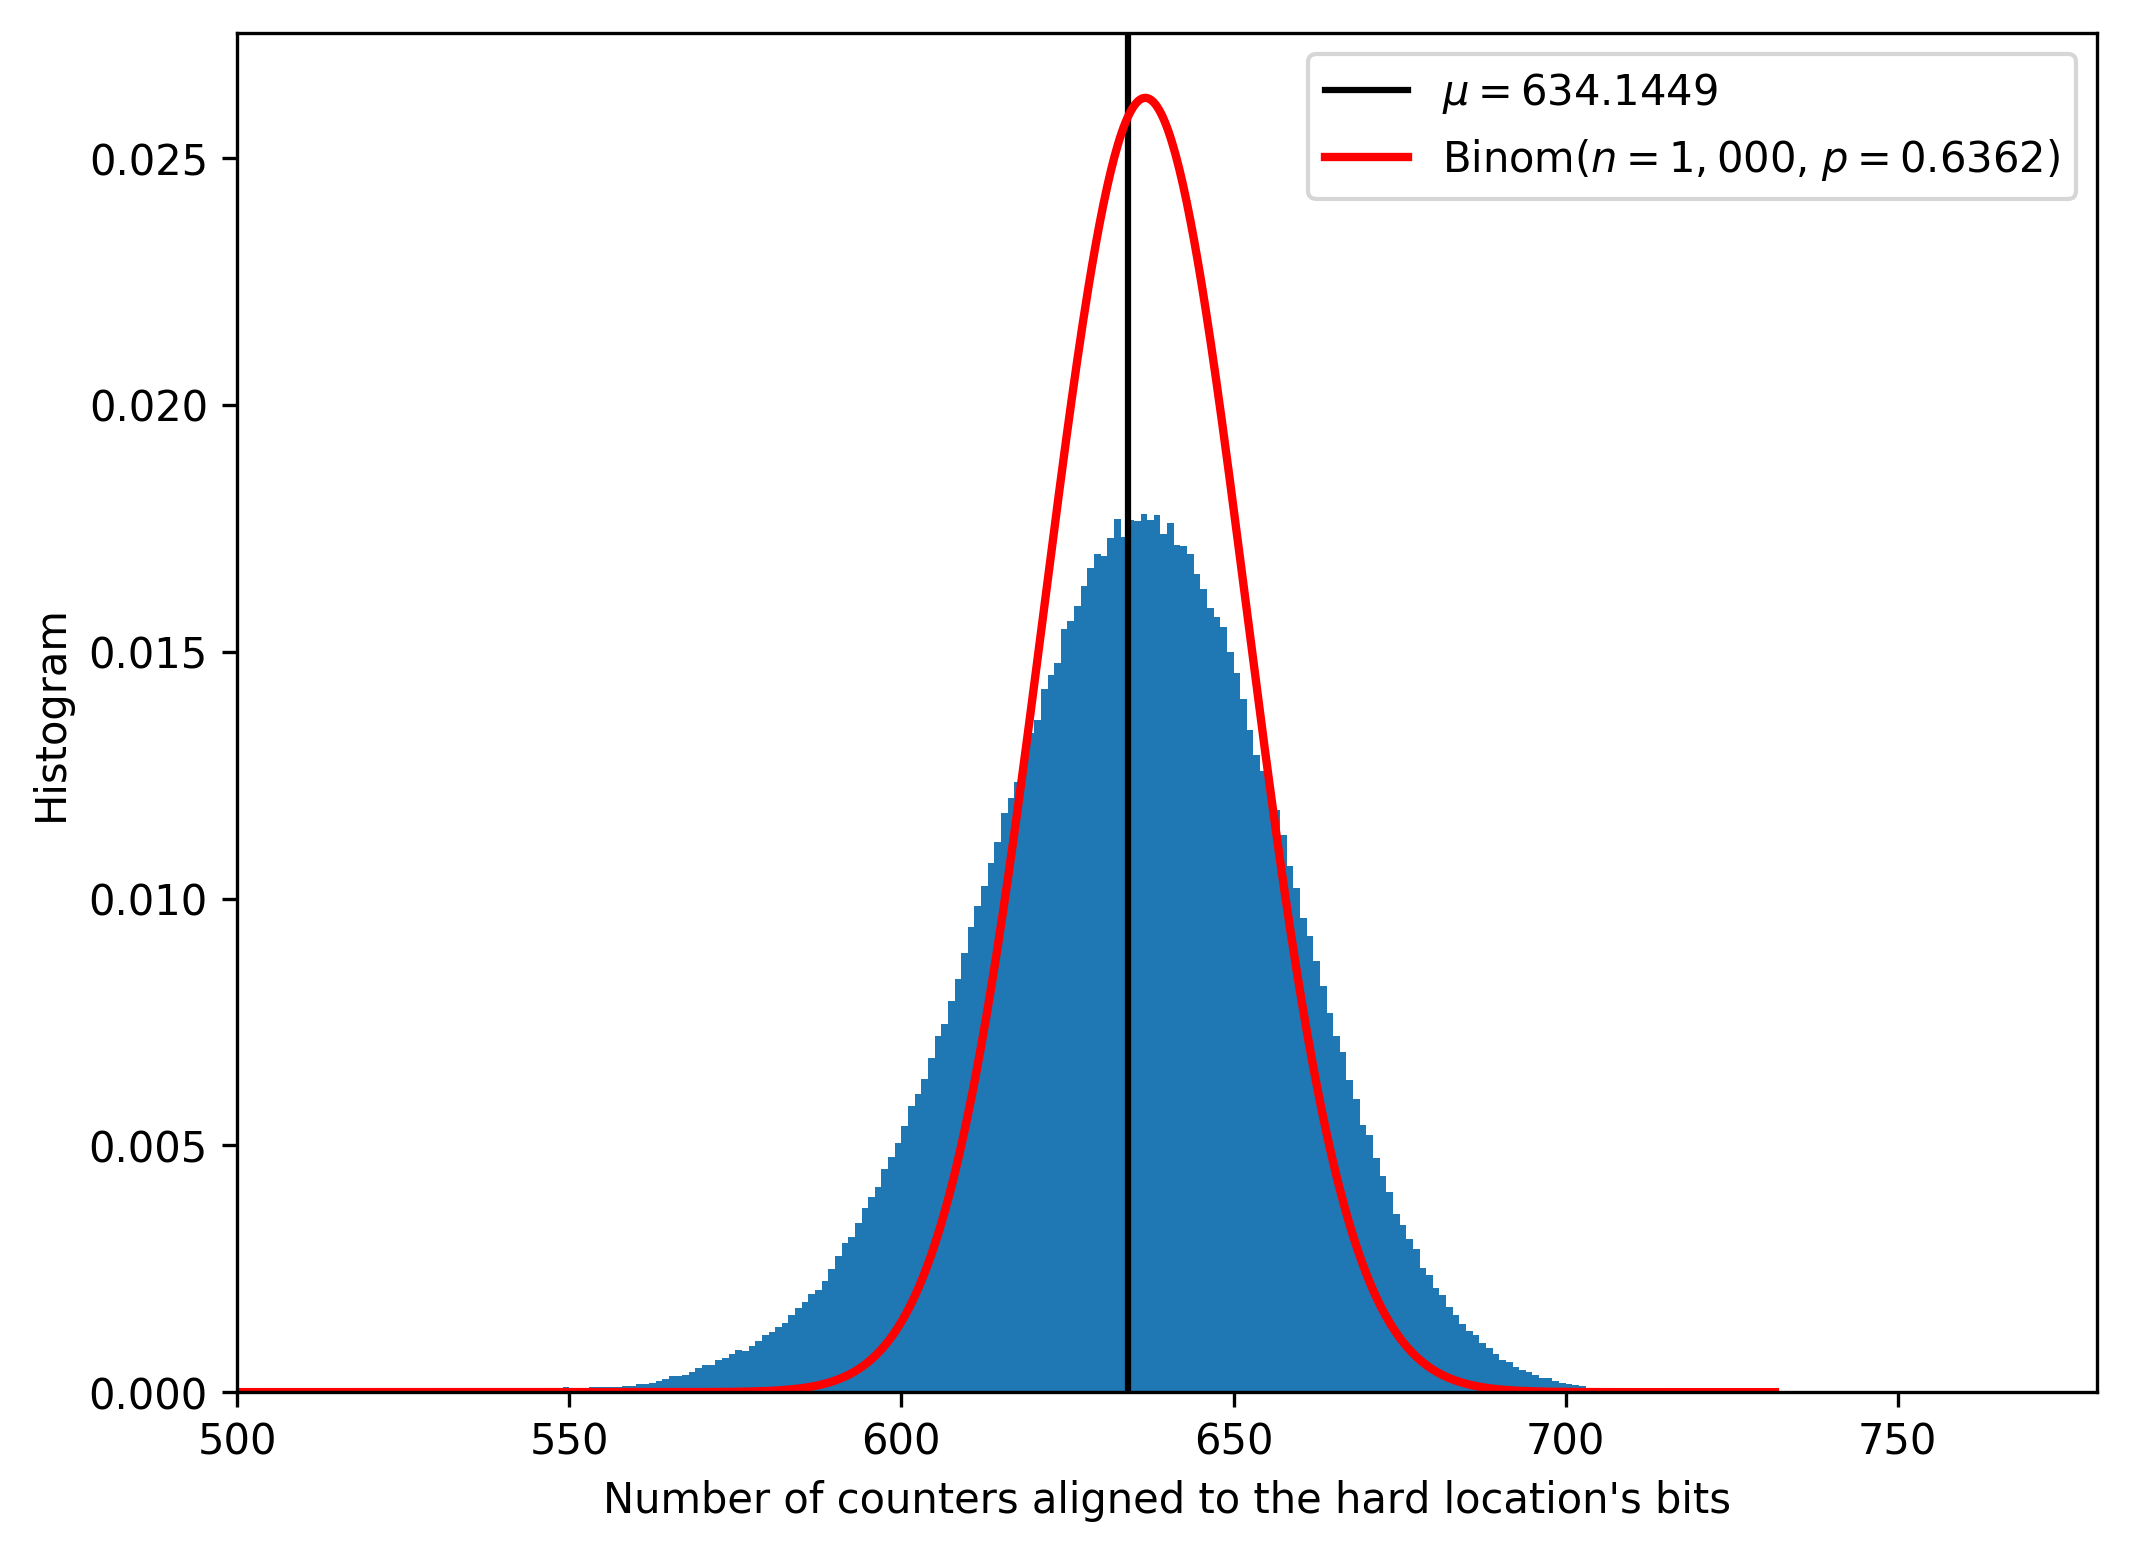
\includegraphics[width=0.5\textwidth]{./images02/autocorrelation/x_at_x_counters.png}}

  \caption{Autocorrelation in the counters in autoassociative memories (``x at x''). The histogram was obtained through simulation. The red curve is the theoretical distribution.}
  \label{fig:sdm-corr-prob}
\end{figure}


Not let's analyze the value of the counters for ``x at x''. In write operation, the counters are incremented for every bit 1 and decremented for every bit 0. So, after $s$ writes, there will be $\theta$ bitstrings written in each hard location, $Y_i = \sum_{k=1}^{\theta} X_k$ bits 1, and $\theta - Y_i$ bits 0. Thus, when $\text{addr}_i = 1$, $\text{cnt}_i = (Y_i) - (\theta - Y_i) = 2Y_i - \theta$. And, when $\text{addr}_i = 0$, $\text{cnt}_i = \theta - 2Y_i$.

As $Y_i \sim \text{Binomial}(\theta, p)$, for $\theta$ sufficiently large, we may approximate $Y_i \sim \mathcal{N}(\mu = \theta p, \sigma^2 = \theta p (1-p))$. Hence, as $\text{cnt}_i = 2Y_i - \theta$, $\mathbf{E}[2Y_i - \theta] = 2 \mathbf{E}[Y_i] - \theta$, and $\mathbf{V}[2Y_i - \theta] = 4 \mathbf{V}[Y_i]$, then,

\begin{align}
\left[ \text{cnt}_i | \text{addr}_i=1 \right] &\sim \mathcal{N}(\mu = (2p-1) \theta, \sigma^2 = 4 \theta p (1-p)) \\
\left[ \text{cnt}_i | \text{addr}_i=0 \right] &\sim \mathcal{N}(\mu = -(2p-1) \theta, \sigma^2 = 4 \theta p (1-p))
\end{align}

In our case, $p=0.5529$, $s=10,000$, $h=1,071.85$, and $H=1,000,000$, so $\theta = 10.7185$ and $\text{cnt}_i \sim \mathcal{N}(\mu=1.1341, \sigma^2 = 10.5985)$. For ``random at x'', $p=0.5$, so $\mu = 0$ and $\sigma^2 = \theta$. See Figure \ref{fig:sdm-corr-counters}.

\begin{figure}[h!]
  \centering
  \subfloat[$\text{addr}_i=1$]{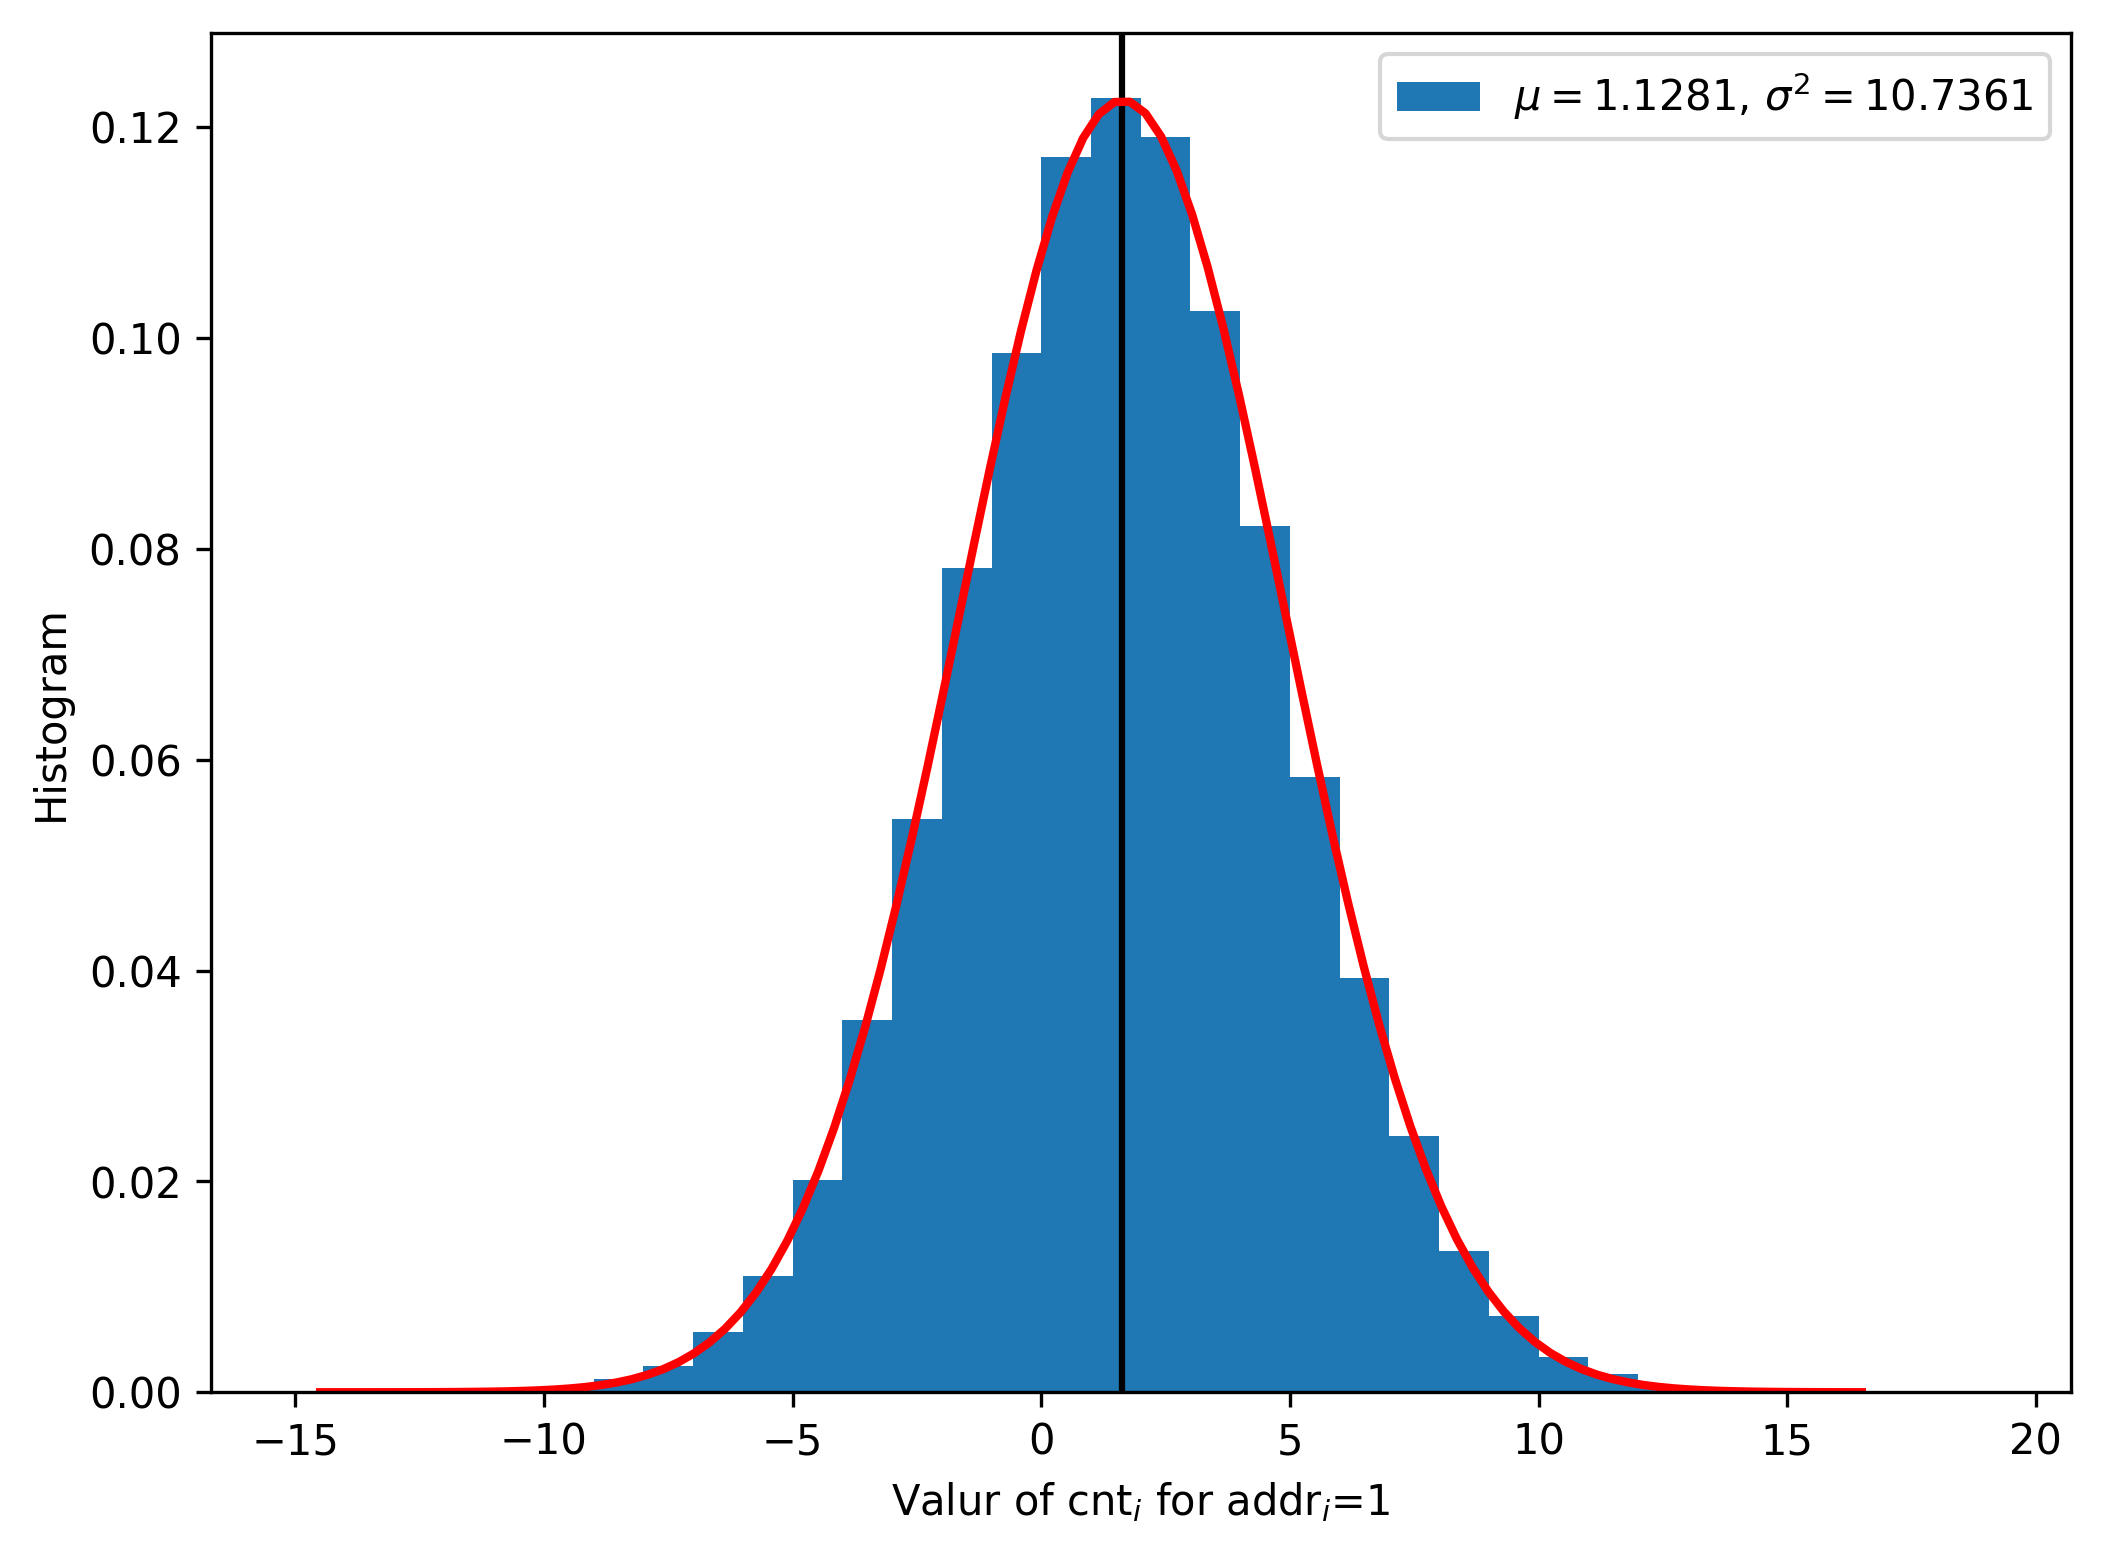
\includegraphics[width=0.5\textwidth]{./images02/autocorrelation/x_at_x_addr1.png}}
  \subfloat[$\text{addr}_i=0$]{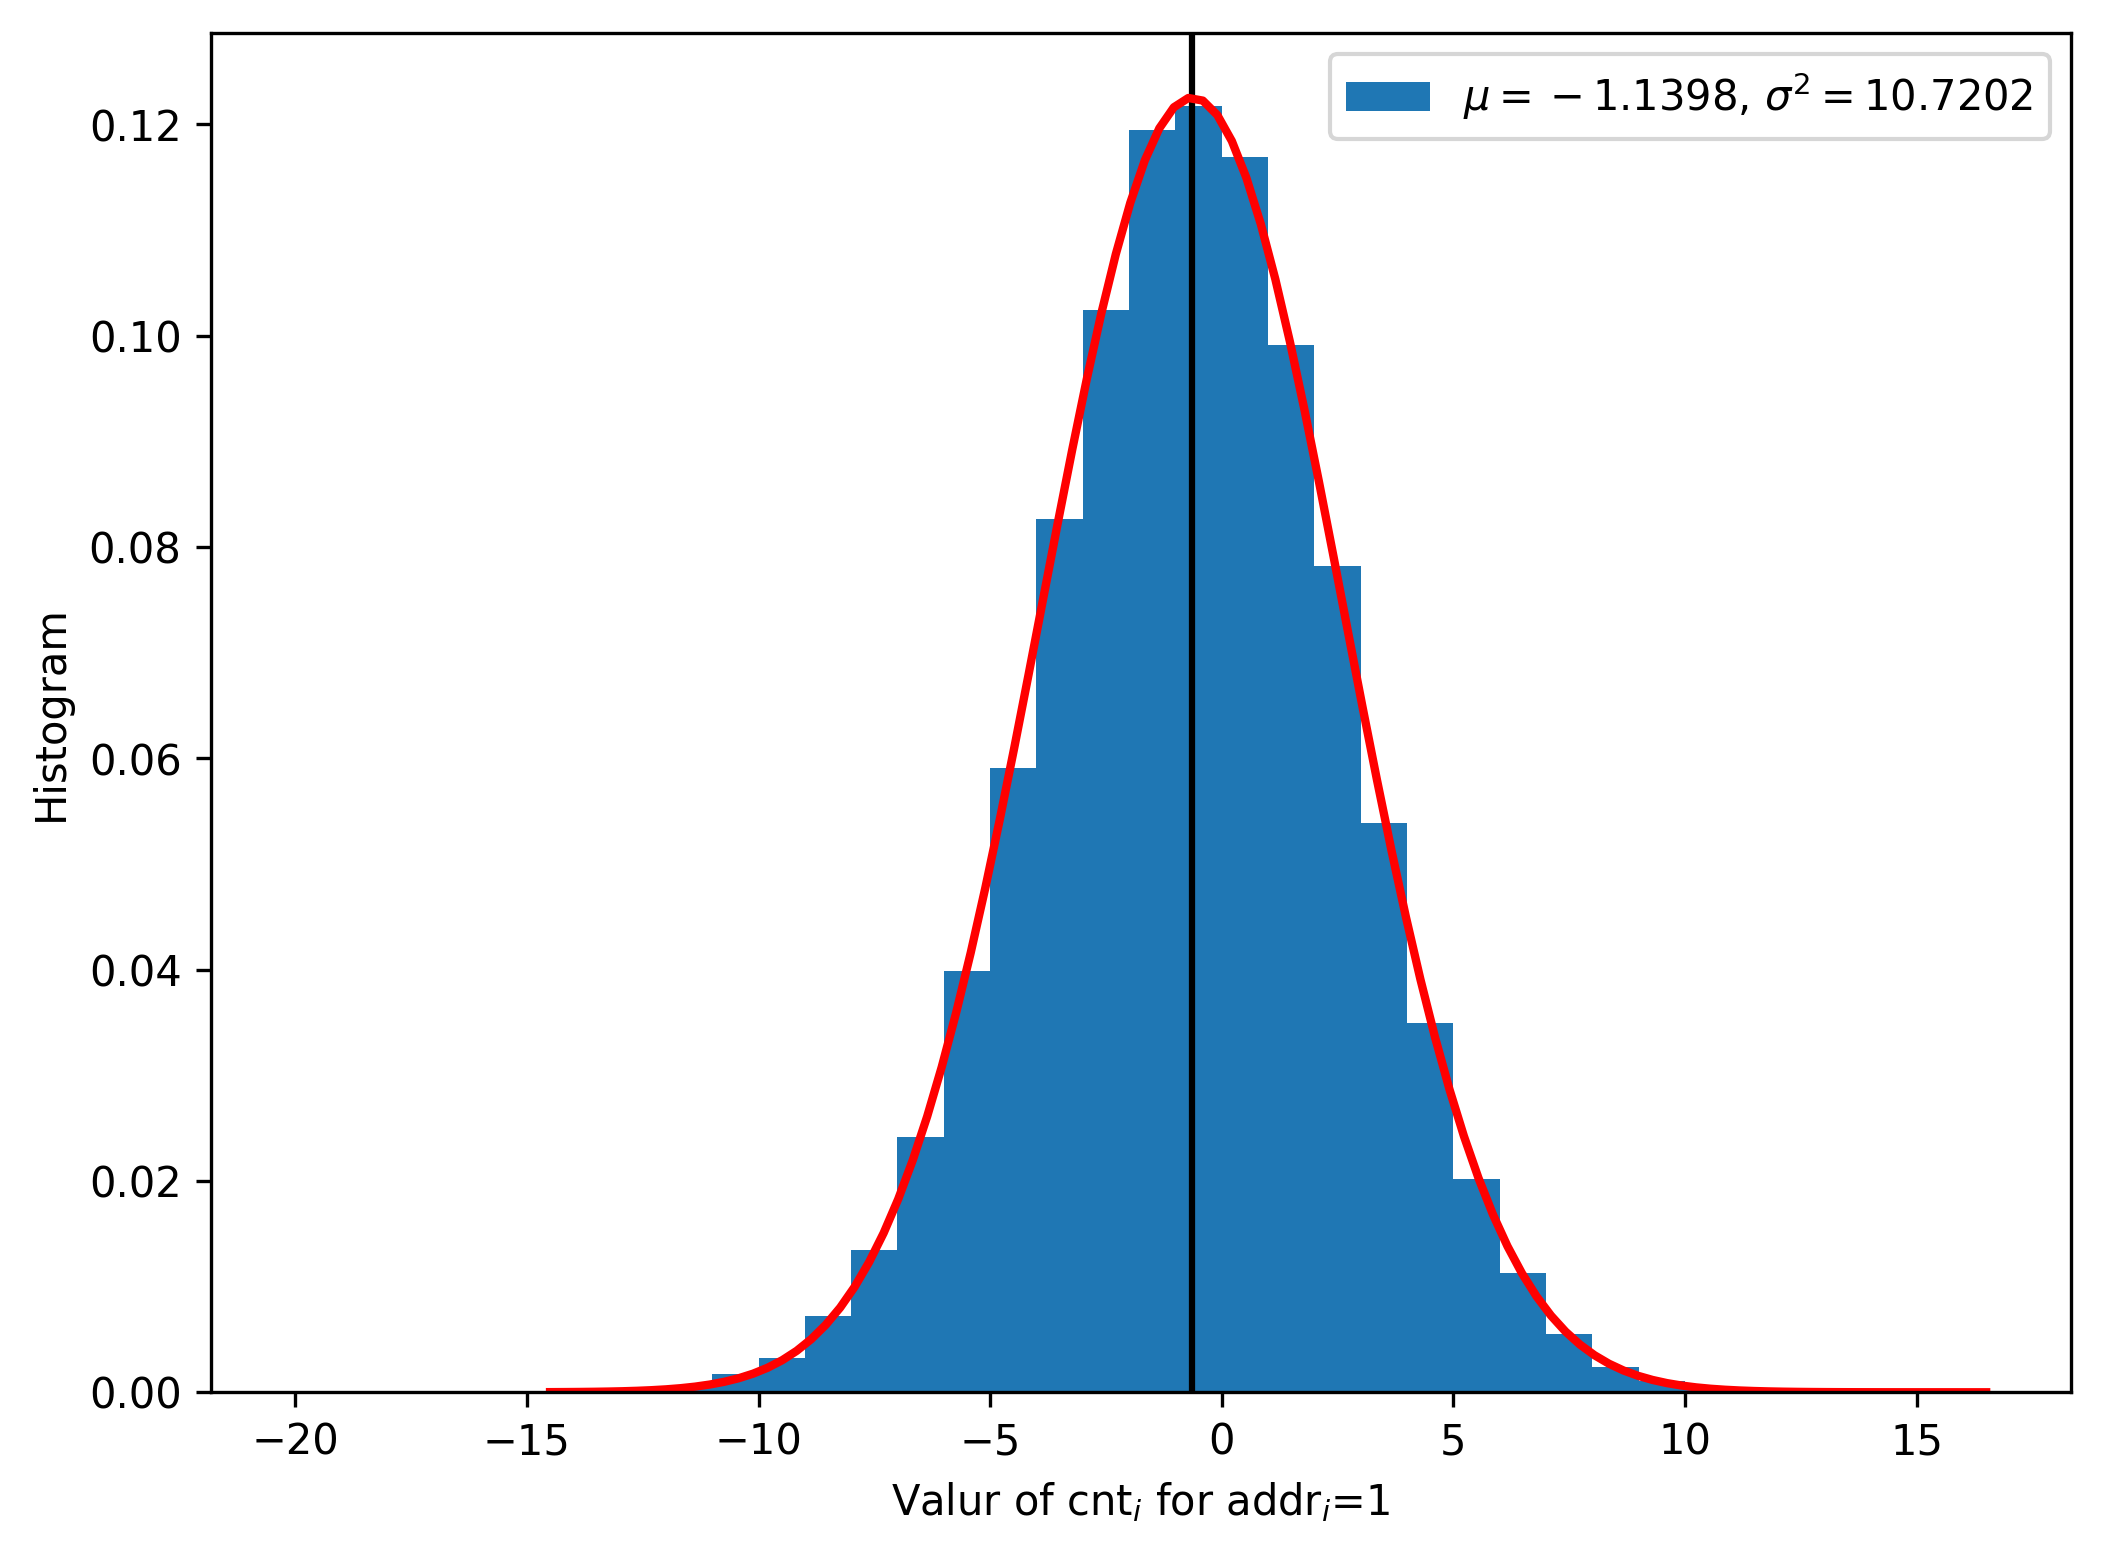
\includegraphics[width=0.5\textwidth]{./images02/autocorrelation/x_at_x_addr0.png}}

  \caption{Autocorrelation in the counters in autoassociative memories (``x at x''). The histogram was obtained through simulation. The red curve is the theoretical normal distribution.}
  \label{fig:sdm-corr-counters}
\end{figure}


\section{Read bias}

Now that we know the distribution of $\text{cnt}_i | \text{addr}_i$, we may go to the read operation. During the read operation, on average, $h$ hard locations are activated and their counters are summed up. So, for the $i$th bit,

\begin{align}
\text{acc}_i = \sum_{k=1}^{h} \text{cnt}_k
\end{align}

Let $\eta$ be the reading address and $\eta_i$ the $i$th bit of it. Then,

\begin{align}
\left[ \text{acc}_i|\eta_i=1 \right] &= \sum_{k=1}^{ph} \left[ \text{cnt}_k | \text{addr}_k=1 \right] + \sum_{k=1}^{(1-p)h} \left[ \text{cnt}_k | \text{addr}_k=0 \right] \\
\left[ \text{acc}_i|\eta_i=0 \right] &= \sum_{k=1}^{ph} \left[ \text{cnt}_k | \text{addr}_k=0 \right] + \sum_{k=1}^{(1-p)h} \left[ \text{cnt}_k | \text{addr}_k=1 \right]
\end{align}

We may analyze only one case, because the probability of the other is exactly the same.

Each sum is a sum of normally distributed random variables, so

\begin{align}
\sum_{k=1}^{ph} \left[ \text{cnt}_k | \text{addr}_k=1 \right] &\sim \mathcal{N}(\mu = (2p-1) \theta ph, \sigma^2 = 4\theta p(1-p) ph) \label{eqn:sdm-eta1-addr1} \\
\sum_{k=1}^{(1-p)h} \left[ \text{cnt}_k | \text{addr}_k=0 \right] &\sim \mathcal{N}(\mu = -(2p-1) \theta (1-p)h, \sigma^2 = 4\theta p(1-p) (1-p)h) \label{eqn:sdm-eta1-addr0}
\end{align}

In our case, $\sum_{k=1}^{ph} \left[ \text{cnt}_k | \text{addr}_k=1 \right] \sim \mathcal{N}(\mu=672.12, \sigma^2=6281.00)$, and $\sum_{k=1}^{ph} \left[ \text{cnt}_k | \text{addr}_k=1 \right] \sim \mathcal{N}(\mu=-543.49, \sigma^2=5078.99)$. See Figure \ref{fig:sdm-read-sums} --- we can notice there a small but significant difference between the theoretical and the simulated mean.

\begin{figure}[h!]
  \centering
  \subfloat[Equation \ref{eqn:sdm-eta1-addr1}  ($\text{addr}_k=1)$]{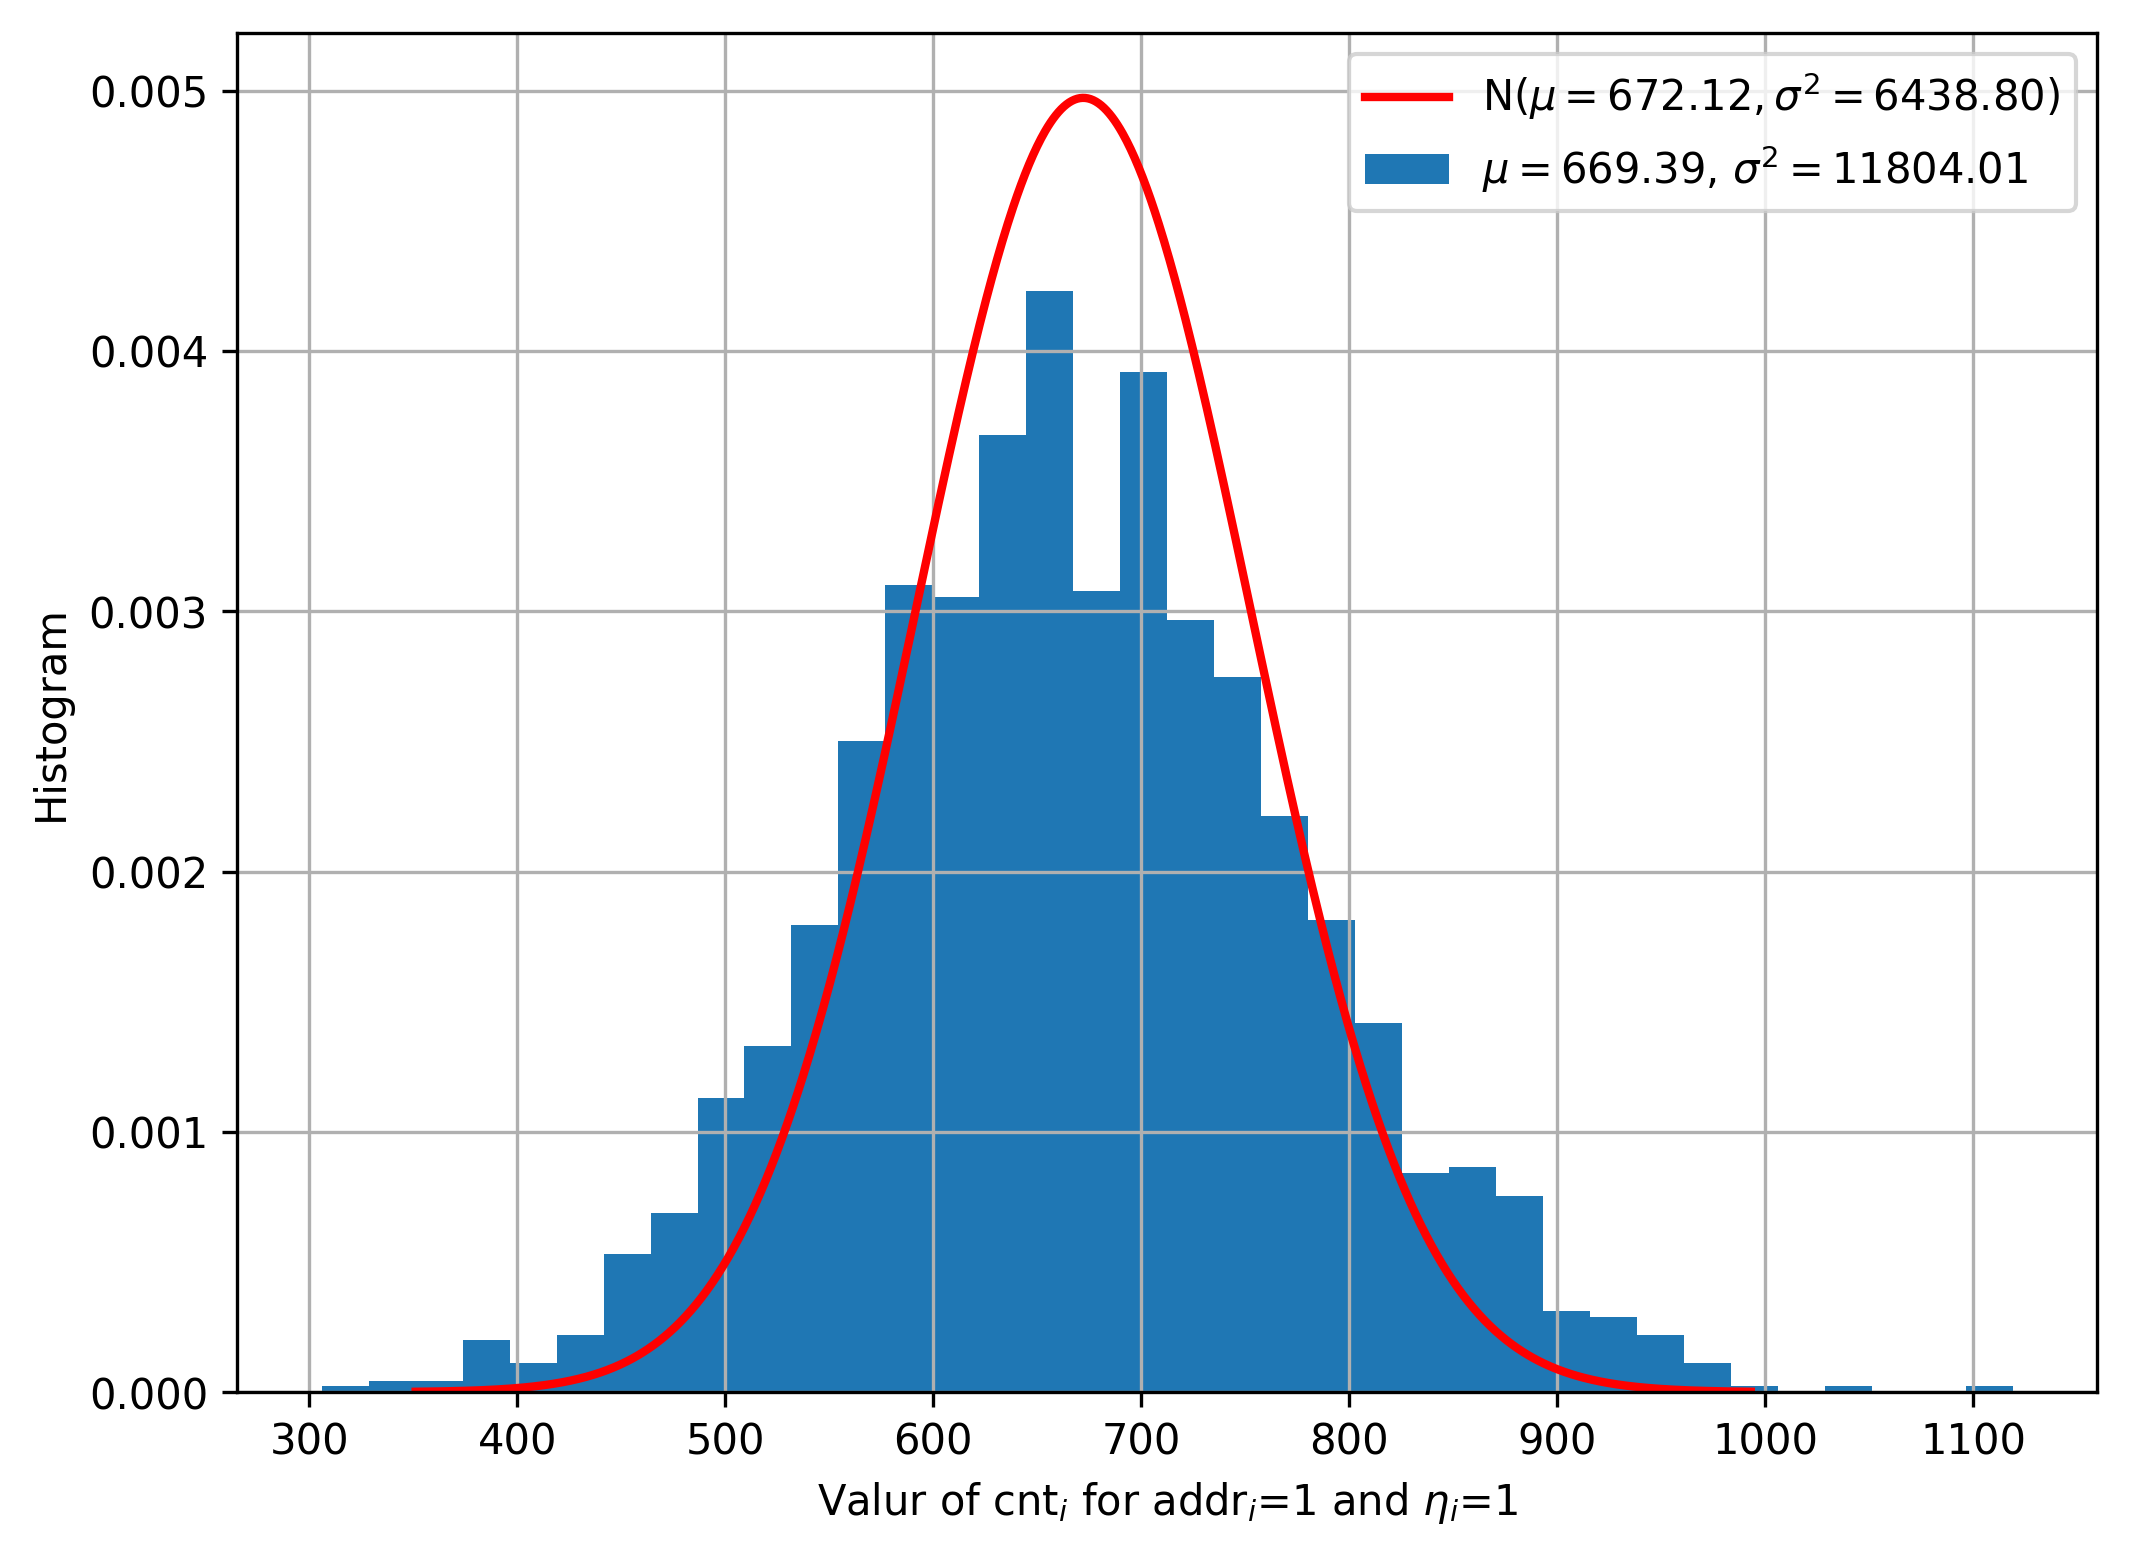
\includegraphics[width=0.5\textwidth]{./images02/autocorrelation/read-counters-eta1_addr1.png}}
  \subfloat[Equation \ref{eqn:sdm-eta1-addr0} ($\text{addr}_k=0$)]{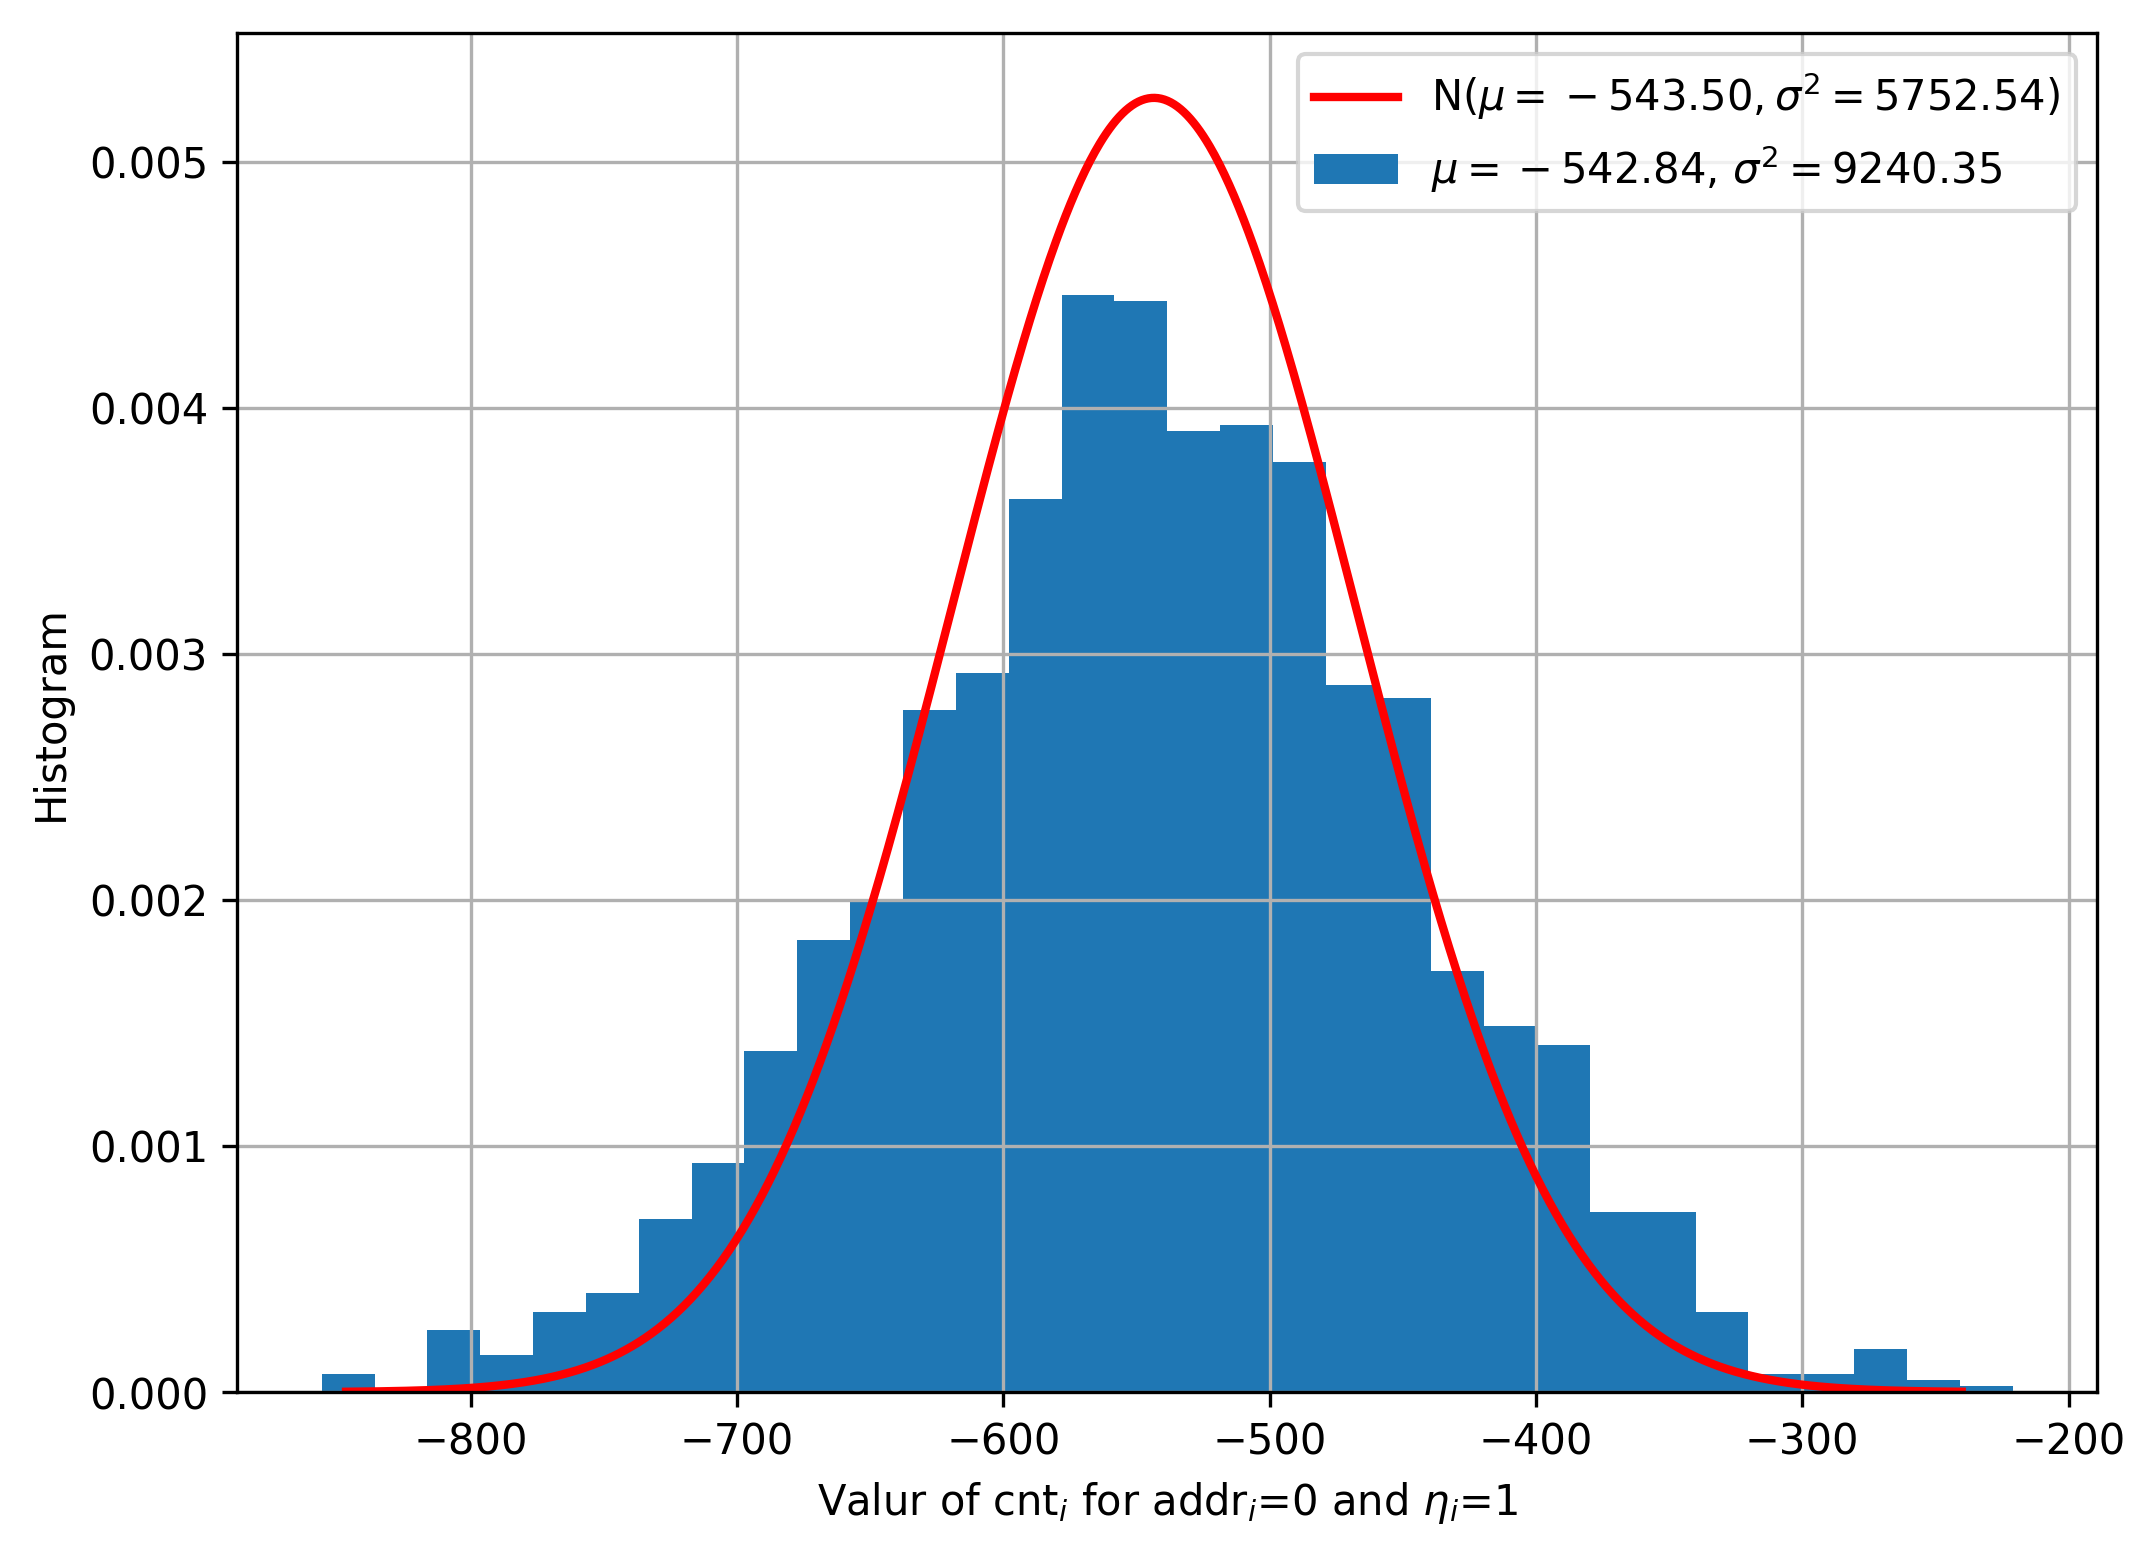
\includegraphics[width=0.5\textwidth]{./images02/autocorrelation/read-counters-eta1_addr0.png}}

  \caption{The histogram was obtained through simulation. The red curve is the theoretical normal distribution.}
  \label{fig:sdm-read-sums}
\end{figure}

Hence,

\begin{align}
\left[ \text{acc}_i|\eta_i=1 \right] &\sim \mathcal{N}(\mu = (2p-1)^2 \theta h, \sigma^2 = 4 \theta p (1-p) h) \label{eqn:sdm-eta1} \\
\left[ \text{acc}_i|\eta_i=0 \right] &\sim \mathcal{N}(\mu = -(2p-1)^2 \theta h, \sigma^2 = 4 \theta p (1-p) h) \label{eqn:sdm-eta0}
\end{align}

In our case, $\left[ \text{acc}_i|\eta_i=1 \right] \sim \mathcal{N}(\mu = 128.62, \sigma^2 = 11359.99)$, and $\left[ \text{acc}_i|\eta_i=0 \right] \sim \mathcal{N}(\mu = -128.62, \sigma^2 = 11359.99)$. See Figure \ref{fig:sdm-read} --- we can notice that the small difference in the means from Figure \ref{fig:sdm-read-sums} has propagated to these images.

\begin{figure}[h!]
  \centering
  \subfloat[Equation \ref{eqn:sdm-eta1}  ($\eta_k=1)$]{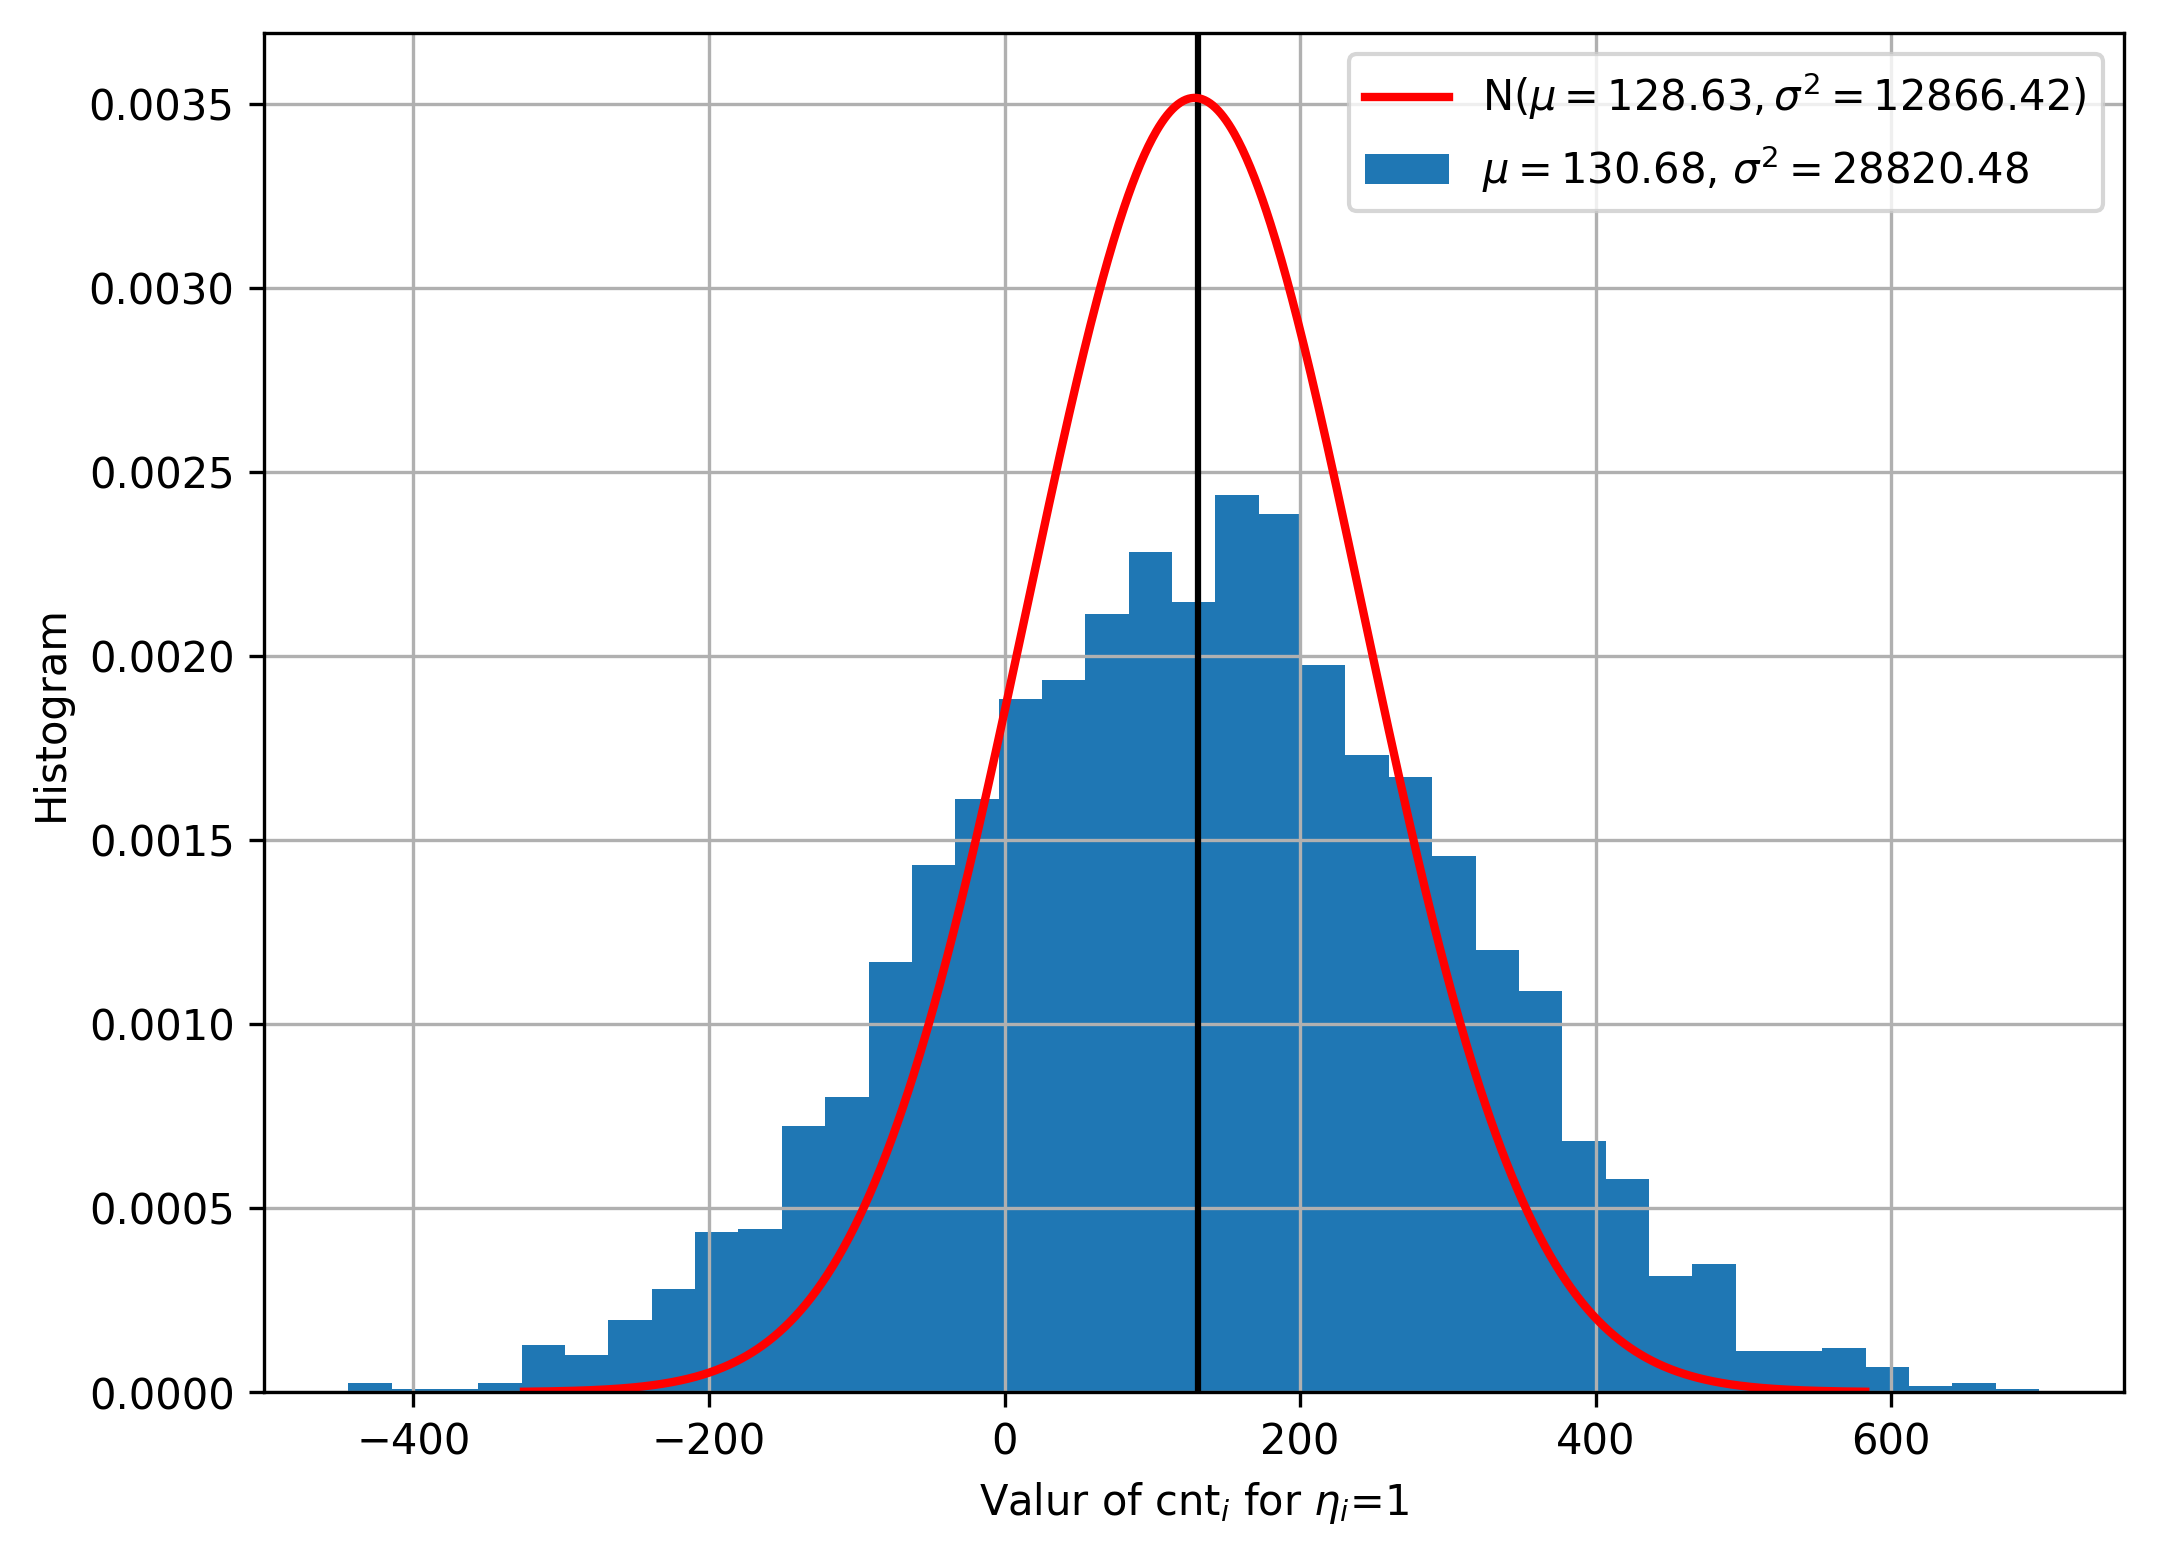
\includegraphics[width=0.5\textwidth]{./images02/autocorrelation/read-counters-eta1.png}}
  \subfloat[Equation \ref{eqn:sdm-eta0} ($\eta_k=0$)]{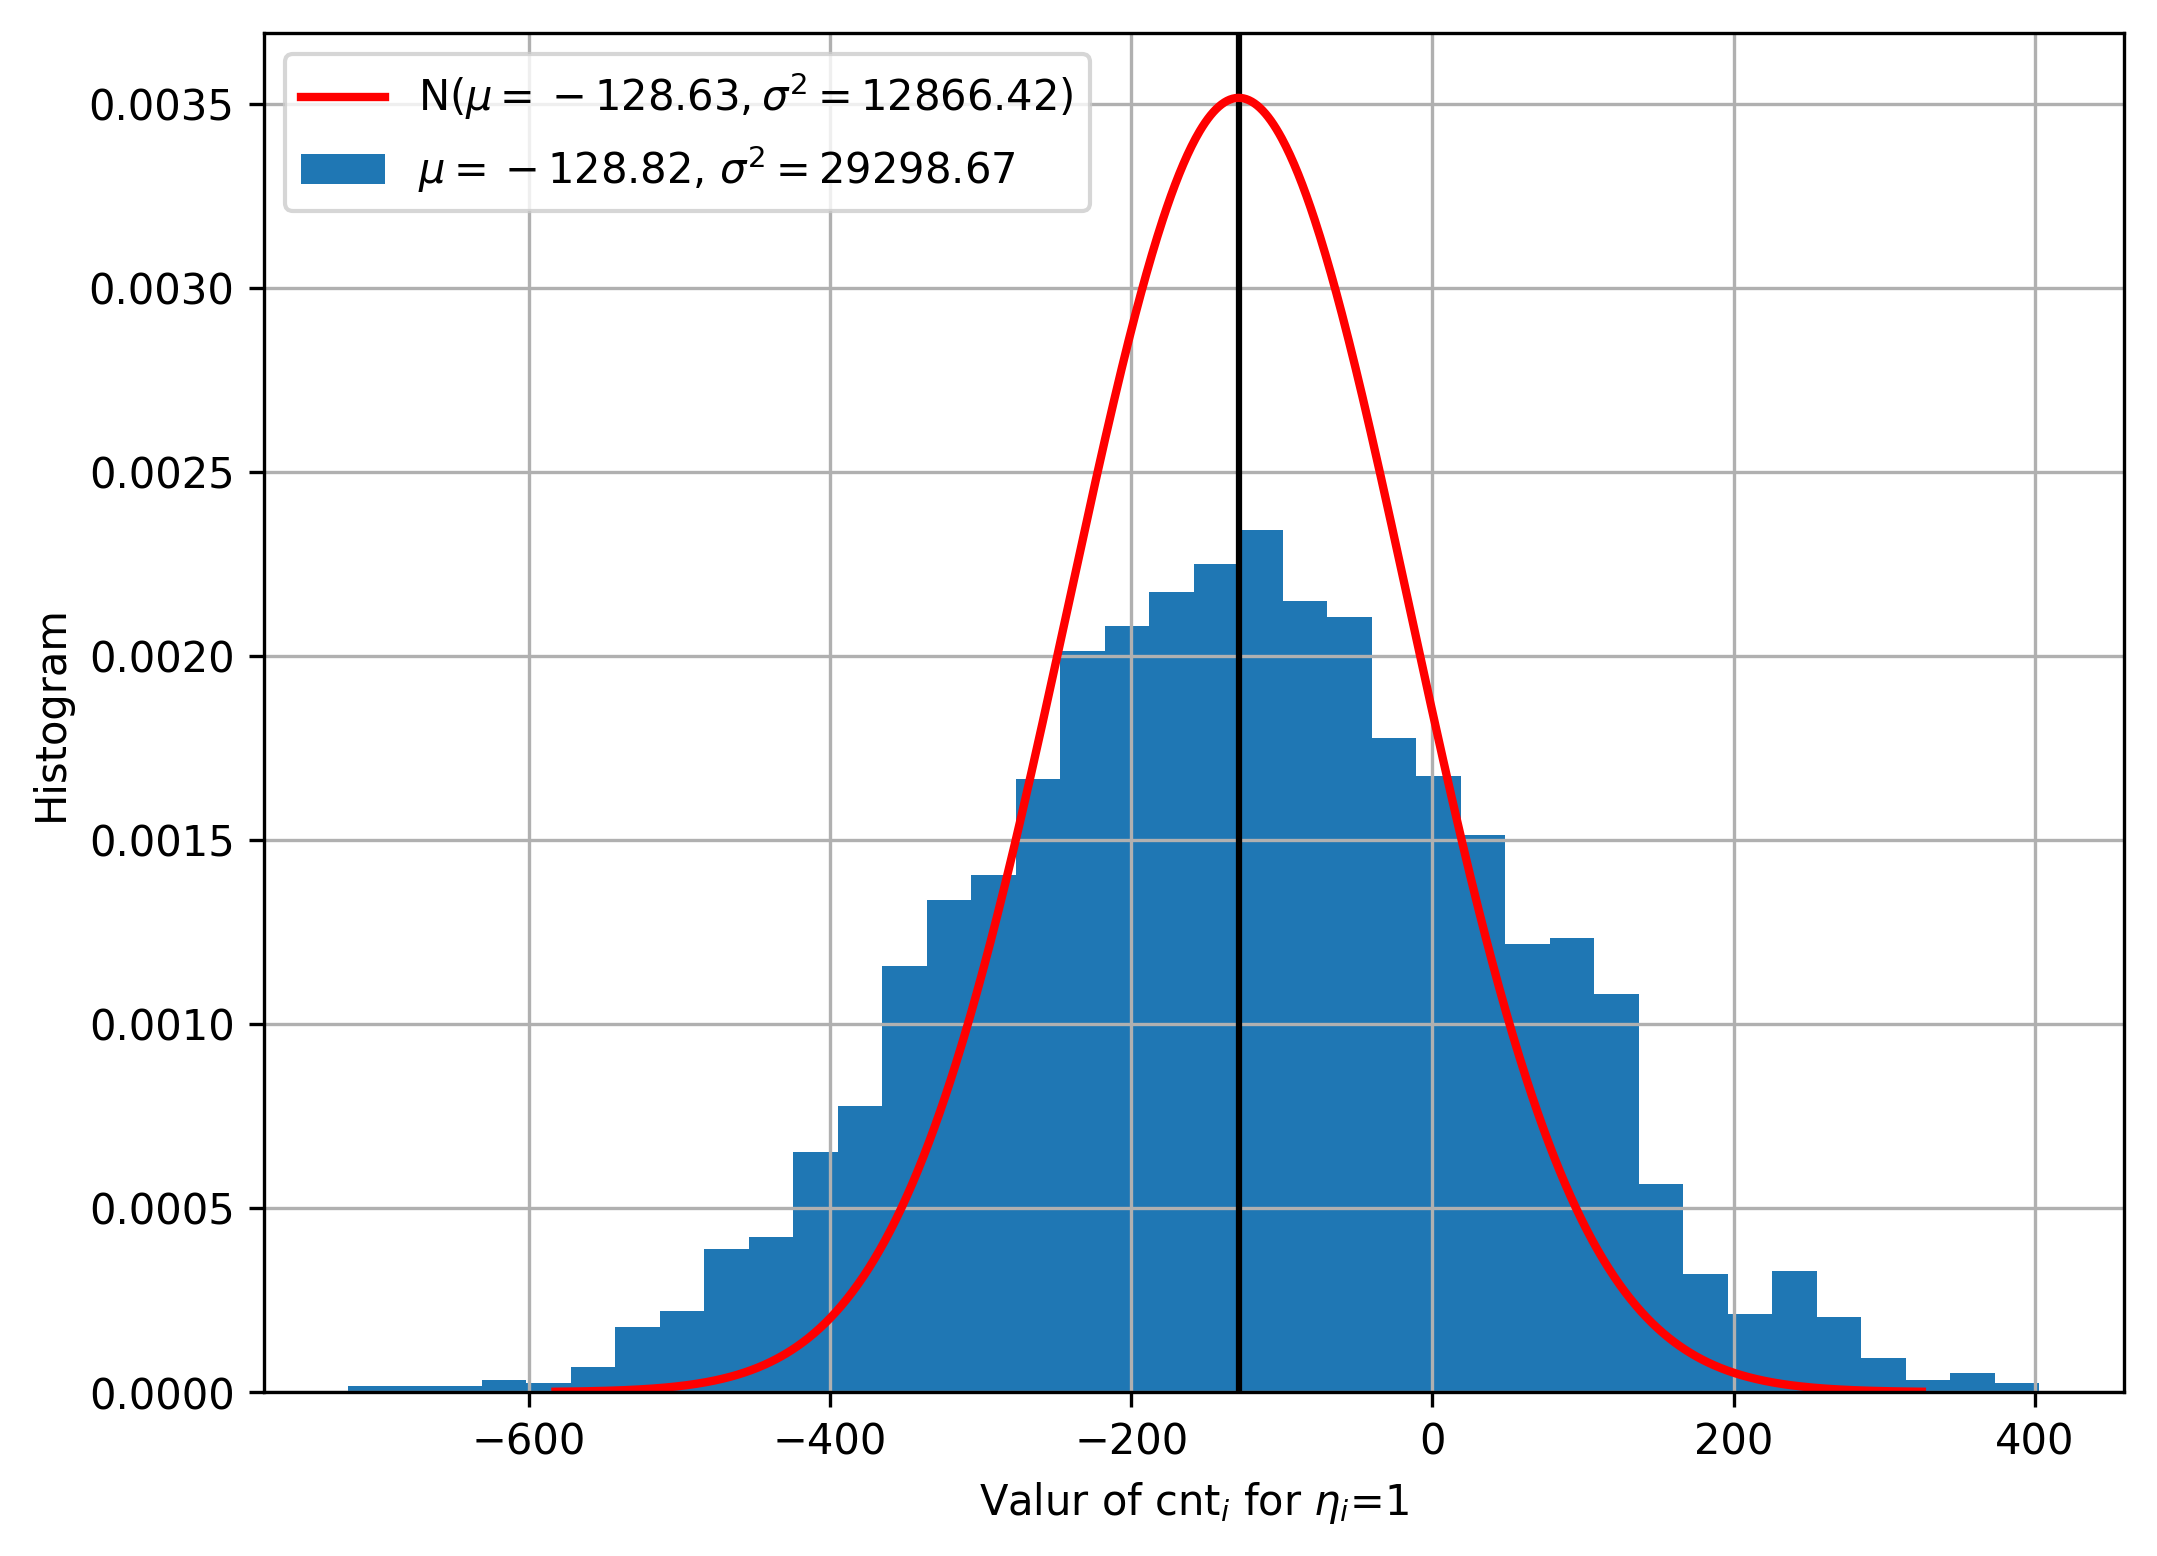
\includegraphics[width=0.5\textwidth]{./images02/autocorrelation/read-counters-eta0.png}}

  \caption{The histogram was obtained through simulation. The red curve is the theoretical normal distribution.}
  \label{fig:sdm-read}
\end{figure}


Finally,

\begin{align}
P(wrong) &= P(\text{acc}_i < 0 | \eta_i = 1) \cdot P(\eta_i = 1) + P(\text{acc}_i > 0 | \eta_i = 0) \cdot P(\eta_i = 0) \\
    &= \frac{\mathcal{N}_{\eta_i=1}.\text{cdf}(0)}{2} + \frac{1-\mathcal{N}_{\eta_i=0}.\text{cdf}(0)}{2} \\
    &= \frac{\mathcal{N}_{\eta_i=1}.\text{cdf}(0)}{2} + \frac{\mathcal{N}_{\eta_i=1}.\text{cdf}(0)}{2} \\
    &= \mathcal{N}_{\eta_i=1}.\text{cdf}(0)
\end{align}

In our case, $P(wrong) = 0.1137518032308093$.

In order to check this probability, I have run a simulation reading from 1,000 random bitstrings (which have never been written into memory) and calculate the distance from the result of a single read. As the $P(wrong) = 0.11375$, I expected to get an average distance of 113.75 with a standard deviation of 10.04. See Figure \ref{fig:sdm-read-random-bs} --- We can notice a big difference between the theoretical model and the simulation. Using $\mu=102$ and $\sigma=121$, the curves match. I'm still looking for the mistake in the equations. I believe the problem is in Equation \ref{eqn:sdm-eta1-addr1}.

\begin{figure}[h!]
  \centering
  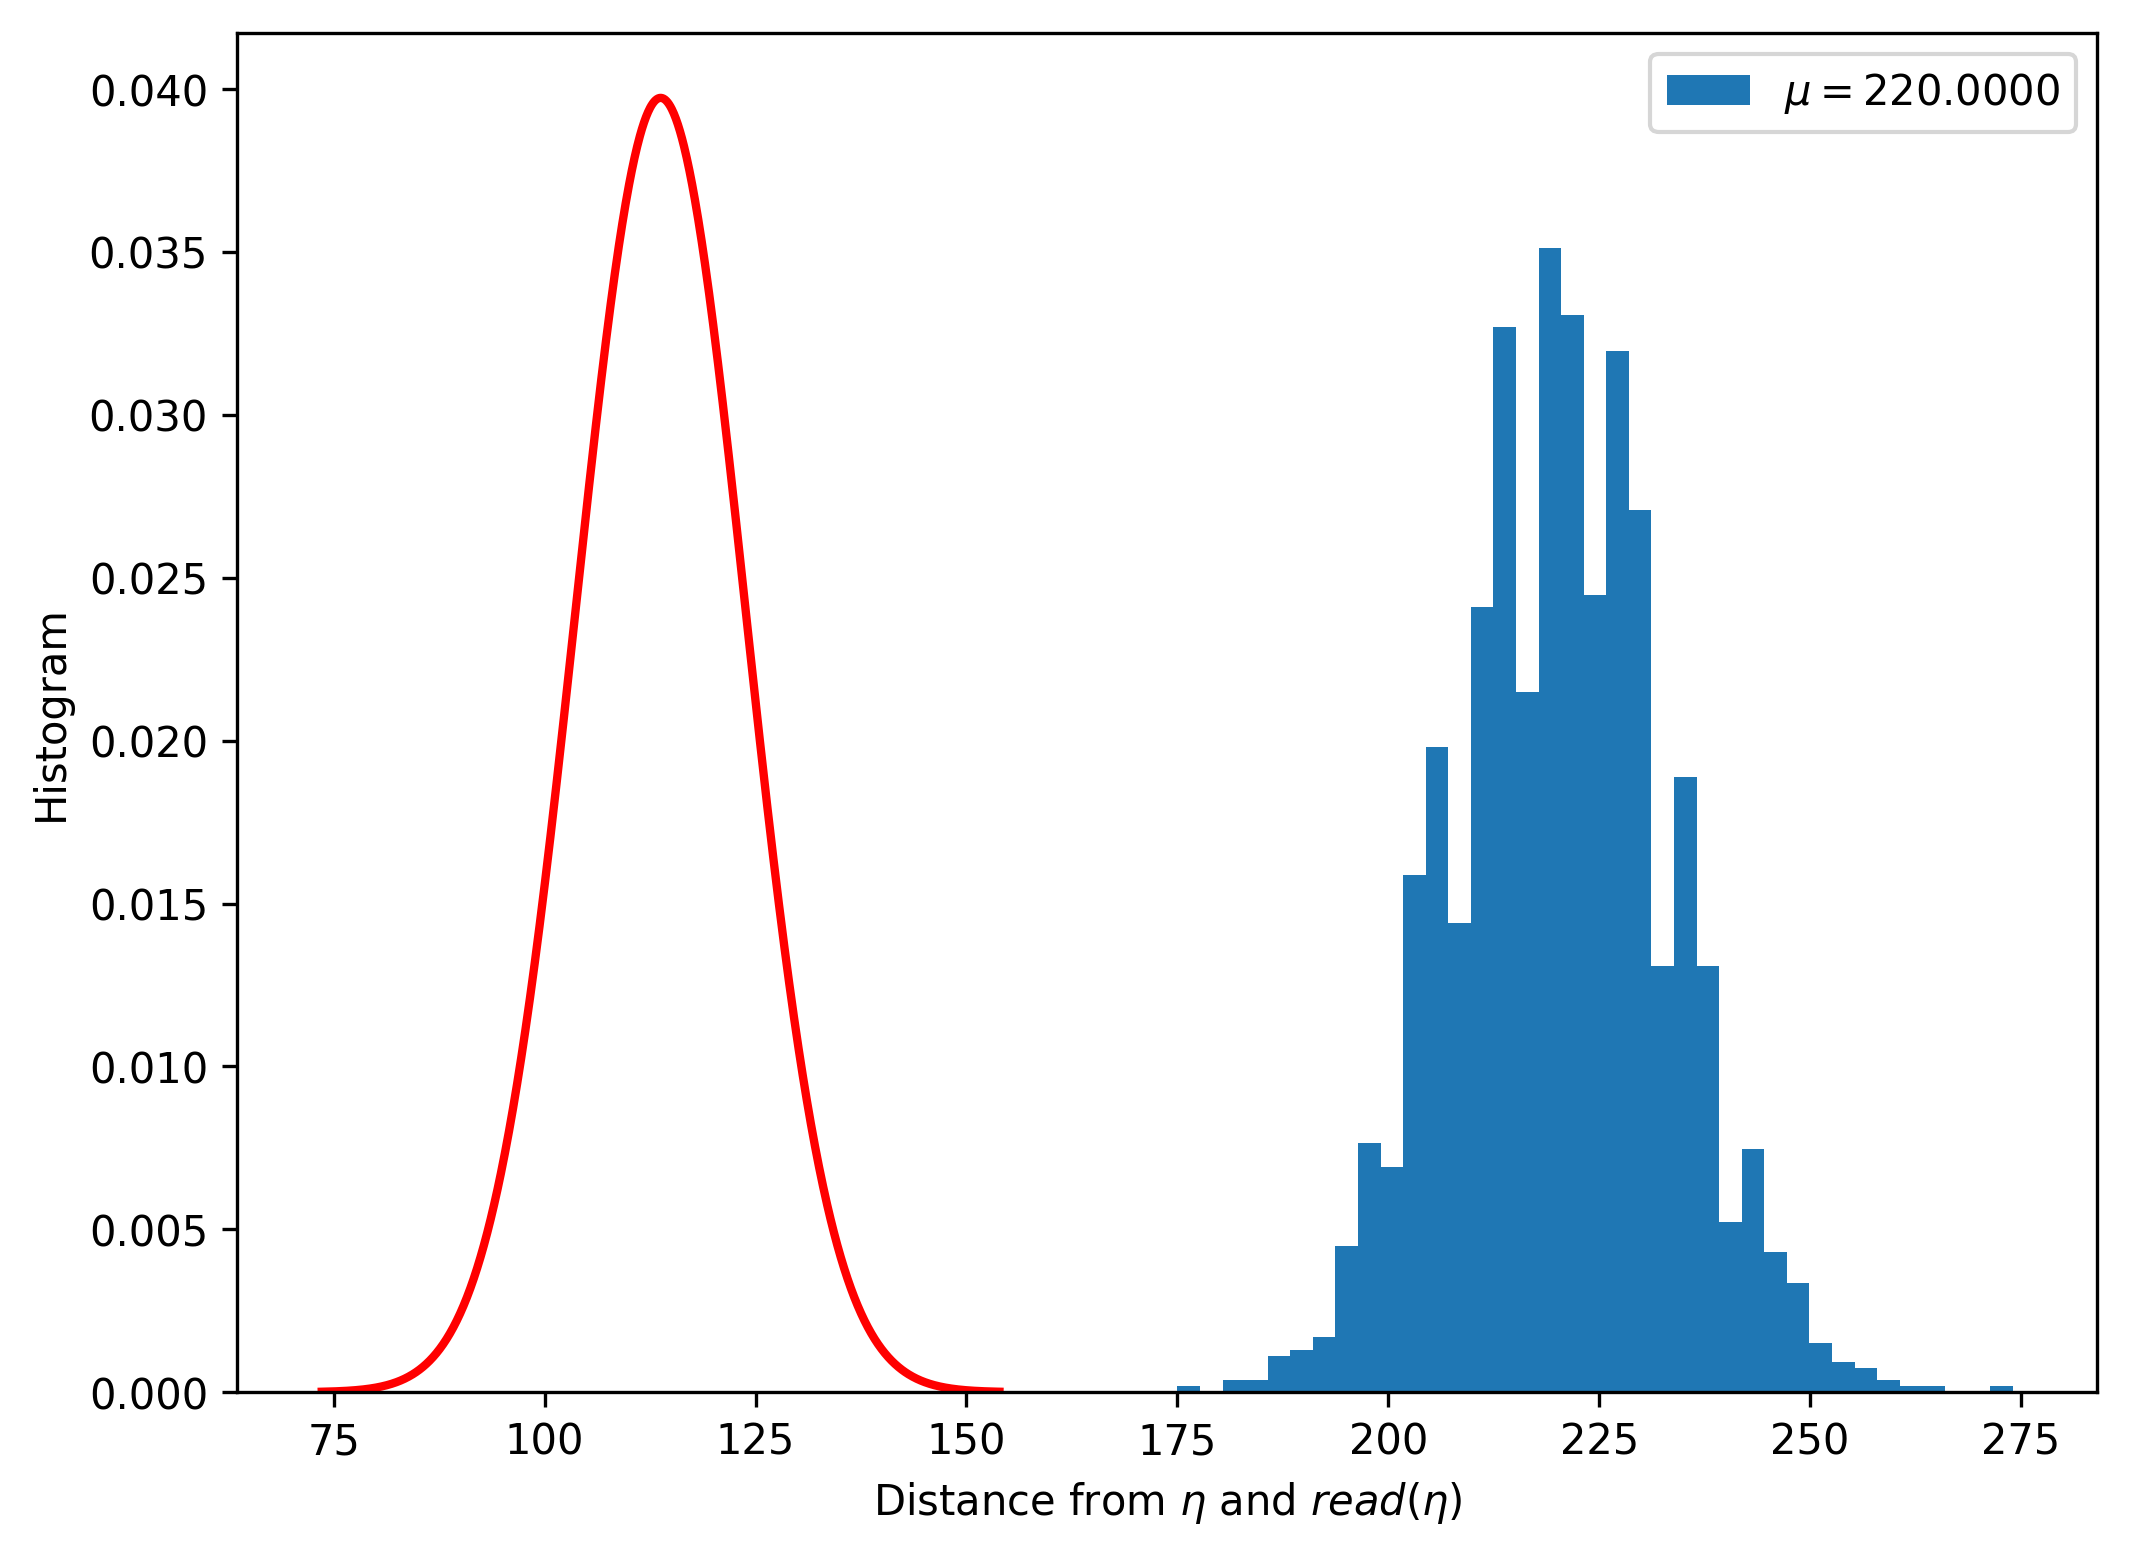
\includegraphics[width=0.75\textwidth]{./images02/autocorrelation/read-random-bs.png}

  \caption{The histogram was obtained through simulation. The red curve is the theoretical normal distribution.}
  \label{fig:sdm-read-random-bs}
\end{figure}


\end{document}
